%!TEX root = main.tex
\blk{rampgen} generates a rising ramp on its output \sig{measure} or maintains it based on its first input \sig{charge}. The second input \sig{start} allows to reset the output to ground.

\subsection{Principle of Operation}
To generate a voltage ramp on command, we choose to charge a capacitor through a switch with a DC current source.

We choose to split the switching and current generation responsibilities between two transistors.
This allows to simulaneously achieve good switching behaviour which requires a low area transistor to reduce the gate parasitic capacitances, and good current source behaviour which requires a long transistor (and thus wide for a given $I_{ds}$ and $V_{ov}$) to reduce $g_{ds}$.

We choose to reference \sig{measurement} to ground so that its scales positively with the measured delay.
This means that one of the capacitor terminals is grounded, and that the current source uses a PMOS.
This choice is arbitrary, but will be taken into account when designing the output stage in order to maximize the output range.

The ramp switching is done using a PMOS as well because it allows to put the source on the drain of the current source which has relatively stable voltage. This gives better results than using an NMOS, because in that case the voltage a the source of the switch is actually the output ramp which should cover the widest possible range of voltages.

Finally, the output is shorted to ground by an NMOS switch controlled by \sig{start}. \sig{start} is thus active-high while \sig{charge} is active-low, which corresponds to what we use in the previous section.

Figure~\ref{fig:rampgen} shows the circuit designed according to these considerations.
\begin{figure}
  \centering
  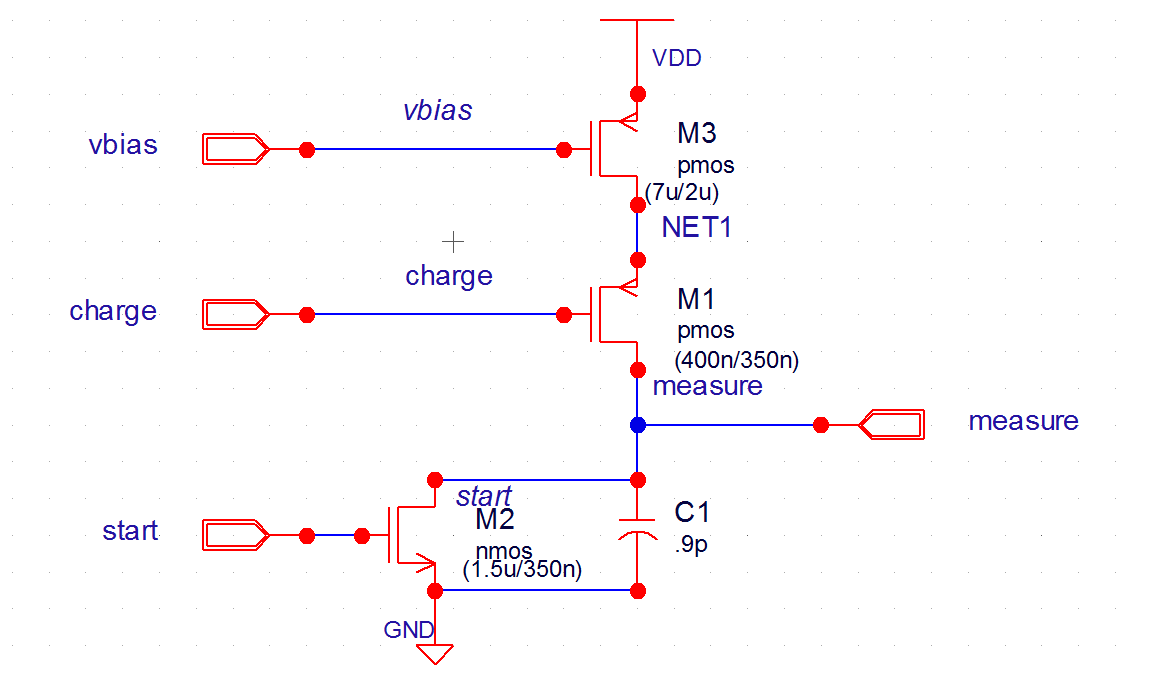
\includegraphics[width=\textwidth]{rampgen.png}
  \caption{\blk{rampgen} Circuit.\label{fig:rampgen}}
\end{figure}

\subsection{Sizing}
\sig{M3} should be long in order to minimize its $g_{ds}$ since it acts as a current source.
Its width, in combination with the capacitance of \sig{C1} determines the slope of the output ramp.
The slope is chosen so that the device reaches the limits of saturation for the longest required delay of \SI{500}{\nano\second}.
The width also controls the sizing of \sig{M1} which has the same $i_{ds}$ as \sig{M3}.

On the other hand, \sig{M1} should be as small as possible for two reasons.
It should be small enough so that it can be correctly driven by \blk{logic}, and it should be as small as possible in order to minimize $C_{gd}$.
${C_{gd}}_{\sig{M3}}$ tends to reproduce the falling and rising edges of \sig{charge} on \sig{measure}, which introduces small steps at the beginning end the end of the output ramp.
This is undesired and increasing \sig{C1} can also reduce this effect.

Based on this, the reasoning that led to the sizing of \sig{M1}, \sig{M3} and \sig{C1} is as follows.
\sig{M3}'s length is set to \SI{2}{\micro\meter} in order to get a good current source behaviour.
A minimally sized transistor can still conduct a reasonable amount of current so we try to use one for \sig{M1}.
\sig{C1} is then set to a value which is big enough to satisfyingly reduce the effect of ${C_{gd}}_{\sig{M3}}$.
Next, ${i_{ds}}_{\sig{M3}}$ is set by choosing \sig{M3}'s width so that the ramp reaches the upper limit of the output range for a \SI{500}{\nano\second} delay.

Finally, we check that \sig{M1} is able to deliver this final value of $i_{ds}$.
A minimally sized transistor is able to deliver the current required by \sig{M3} so the sizing of this part of the ciruit is finished.

For \sig{M2}, we don't care about linearity so we use a minimal length transistor that is wide enough to reset \sig{measure} to ground in \SI{10}{\nano\second}, the length of a pulse, so that the output is properly initialized for the next measurement.
